\documentclass[12pt,a4paper]{article}
\usepackage[utf8]{inputenc}
\usepackage[english]{babel}
\usepackage{amsmath}
\usepackage{amsfonts}
\usepackage{amssymb}
\usepackage{graphicx}
\usepackage{pgfplots}
\pgfplotsset{compat=1.13}
\newcommand{\ratelaw}{\theta(\mathbf{s},\mathbf{p})}
\renewcommand*\rmdefault{bch}


\begin{document}
\section{Control Theory}
\subsection{What is elasticity?}
Metabolic Control Analysis \cite{Fell1996-be} is a mathematical framework that is widely used to dynamic systems such as metabolic networks. In particular, it defines local properties called elasticities that can be used to quantify the control of some variables, such as fluxes, depend on other features of the system. The \emph{scaled elasticity} is the infinitesimal response of a single flux ($v$) to one of the parameters ($a$), using a partial derivative of the log-scaled functions:
\begin{eqnarray}
    \epsilon_a^v \equiv \frac{\partial \ln(v)}{\partial \ln(a)} = \frac{\partial v}{\partial a} ~ \frac{a}{v}
\end{eqnarray}

\subsection{Single-substrate Control}
Consider an enzyme-catalyzed reaction, described by a one-substrate irreversible Michaelis-Menten kinetic rate law:
\begin{eqnarray}
    v &=& V^+ ~ \frac{s}{K_M + s}
\end{eqnarray}
where $s$ is the substrate concentrations (in units of molar), and $K_M$ is the Michaelis-Menten coefficient (also in molar).

The scaled elasticities for $s$ and $i$ are given by:
\begin{eqnarray}
    \epsilon_s^v &=& \frac{\partial v}{\partial s} ~ \frac{s}{v} = V_{max} ~ \frac{K_M + s - s}{(K_M + s)^2} ~ \frac{s}{v} \nonumber \\
    &=& \frac{K_M}{(K_M + s)^2} ~ (K_M + s) = \frac{K_M}{K_M + s} = 1 - \frac{s}{K_M + s}\label{eq:eps_s_v_irr}
\end{eqnarray}

As shown in \cite{Noor2013-vv}, this formula for substrate elasticity can be generalized to reversible Michaelis-Menten reactions, where the saturation term is separated from the thermodynamic term:
\begin{eqnarray}
    v &=& V^+ \cdot \kappa \cdot \gamma \\
    \kappa &\equiv& \frac{s/K_S}{1 + s/K_S + p/K_P} \\
    \gamma &\equiv& 1 - \frac{p/s}{K_{eq}'}
\end{eqnarray}
where $p$ is the product concentration, $K_S$ and $K_P$ are the Michaelis-Menten constants for the substrate and product, and $K_{eq}'$ is the apparent equilibrium constant. In this case, the elasticity of the substrate and product are:
\begin{eqnarray}
    \epsilon_s^v &=& \gamma^{-1} - \kappa
\end{eqnarray}
which converges to equation \ref{eq:eps_s_v_irr} as $p \rightarrow 0$.

\subsection{Regulatory Effectors}
As far as we know, previous publications have not dealt specifically with elasticities associated with small-molecule effectors such as allosteric regulators. Without loss of generality, we will keep the separable form of the rate law
\[v = V^+ \cdot \kappa \cdot \gamma \cdot \theta(x)\]
where we add a multiplicative term $\theta(x)$ that will represent the decrease of activity due to the small-molecule regulation ($x$). As long as $\theta(x)$ is the only term affected by $x$, i.e. $\frac{\partial \kappa}{\partial x} = \frac{\partial \gamma}{\partial x} = 0$, the exact forms of $\kappa$ and $\gamma$ are irrelevant.

\subsubsection{Activation}
First, consider a cooperative \cite{Barcroft1910-rx, Monod1965-dq} activator with Hill coefficient $h$ and activation coefficient $K_A$:
\begin{eqnarray}
    \theta &=& \frac{x^h}{K_A^h + x^h}~.
\end{eqnarray}
The elasticity with respect to the activator concentration $x$ will thus be:
\begin{eqnarray}
    \epsilon_x^v &=& \frac{\partial v}{\partial x} ~ \frac{x}{v} = V^+ ~ \kappa ~ \gamma ~ \frac{h~x^{h-1} (K_A^h + x^h) - h~x^{h-1} x^h}{(K_A^h + x^h)^2}~\frac{x}{v} \nonumber \\
    &=& h~\frac{K_A^h}{K_A^h + x^h} = h (1 - \theta) \label{eq:eps_act}
\end{eqnarray}

\subsubsection{Non-competitive Inhibition}
First, consider a non-competitive inhibitor with Hill coefficient $h$ and inhibition coefficient $K_I$:
\begin{eqnarray}
    \theta &=& 1 - \frac{x^h}{K_I^h + x^h} = \frac{K_I^h}{K_I^h + x^h}
\end{eqnarray}

The following plot shows the response of $\theta$ to the concentration $x$ in log-log scale, when the Hill coefficient is $h = 2$.

\begin{center}
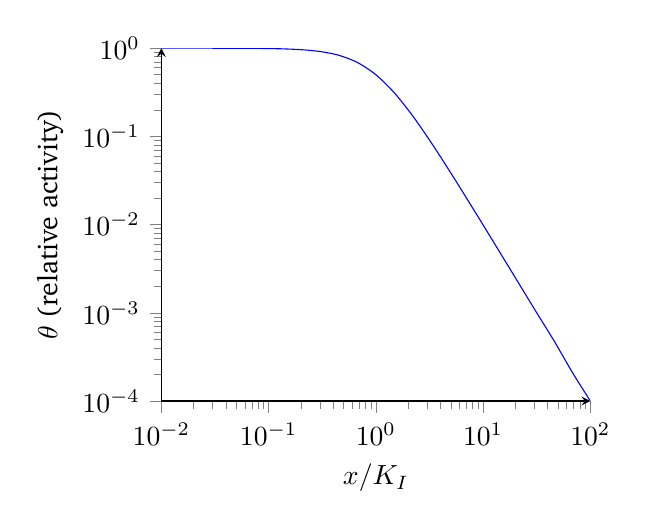
\begin{tikzpicture}
	\begin{loglogaxis}[width=200pt,axis x line=bottom, axis y line=left, tick align=outside, domain=1e-2:1e2, xlabel=$x/K_I$, ylabel=$\theta$ (relative activity)]
		\addplot+[mark=none,smooth] (\x,{(1 - (\x^2/(1+\x^2))});
	\end{loglogaxis}
\end{tikzpicture}
\end{center}

In this case, the elasticity with regards to the inhibitor concentration would be:
\begin{eqnarray}
    \epsilon_x^v &=& \frac{\partial v}{\partial x}\cdot\frac{x}{v} = V^+ ~ \kappa ~ \gamma ~ \frac{- h ~ x^{h-1}}{(K_I^h + x^h)^2} ~ \frac{x}{v} \nonumber \\
    &=& -\frac{h ~ x^h ~ (K_I^h + x^h)}{(K_I^h + x^h)^2} = -h ~ \frac{x^h}{K_I^h + x^h} = -h (1 - \theta)~. \label{eq:eps_inh}
\end{eqnarray}

Plotting the elasticity as a function of $x$, we see that it is a monotonically decreasing negative function:

\begin{center}
\begin{tikzpicture}
	\begin{semilogxaxis}[width=200pt,axis x line=bottom, axis y line=left, tick align=outside, domain=1e-2:1e2, xlabel=$i/K_I$, ylabel=$\epsilon_x^v$]
		\addplot+[mark=none,smooth] (\x,{-2 * (\x^2/(1+\x^2))});
	\end{semilogxaxis}
\end{tikzpicture}
\end{center}

This means that substrates have the most control ($\epsilon_s^v \rightarrow 1$) when they are much below saturation ($s \ll K_M$) while inhibitors have the most control ($\epsilon_x^v \rightarrow -h$) when they are saturated ($i \gg K_I$).


\subsubsection{Competitive Inhibition}
Competitive inhibition is a special case, where a separable kinetic rate law is not sufficient since $\frac{\partial \kappa}{\partial x} \neq 0$. To analyze this case, we pick a simple one-substrate irreversible reaction, where the inhibitor affects the $K_M$ according to the following formula:
\begin{eqnarray}
    v &=& V^+ ~ \frac{s}{K_M \left(1 + \frac{x^h}{K_I^h}\right) + s}
\end{eqnarray}
In this case, we can define an \emph{effective} inhibition constants $K_E$, that will allow us to rewrite this rate law in a form identical to non-competitive inhibition:
\begin{eqnarray}
    K_E &\equiv& K_I \sqrt[h]{\frac{K_M + s}{K_M}} \nonumber\\
    v &=& V^+ ~ \frac{s}{K_M \left(1 + \frac{x^h}{K_I^h}\right) + s} =
          V^+ ~ \frac{s}{K_M \left(1 + \frac{x^h~(K_M + s)}{K_E^h~K_M}\right) + s} = \nonumber\\
      &=& V^+ ~ \frac{s}{K_M + s + \frac{x^h~(K_M + s)}{K_E^h}} = 
          V^+ ~ \frac{s}{K_M + s} \cdot \frac{1}{1 + \frac{x^h}{K_E^h}} \label{eq:eps_comp_inh}
\end{eqnarray}
so we can see here that in this case $\theta = \frac{K_E^h}{K_E^h~+~x^h}$, exactly like in the case of non-competitive inhibition. Of course, the difference here is that $K_E$ is not a binding constant but rather a function of $s$ and $K_M$. Nevertheless, we can use the same formula for the elasticity (since $K_E$ is a constant with regards to $x$):
\begin{eqnarray}
    \epsilon_x^v &=& \frac{\partial v}{\partial x}~\frac{x}{v} = -h(1 - \theta)
\end{eqnarray}

\subsection{A Trade-off between Enzyme Cost and Flux Control}
By taking the absolute value of the elasticity, we can compress the results for activators (Equation \ref{eq:eps_act}) and inhibitors (Equations \ref{eq:eps_inh} and \ref{eq:eps_comp_inh}) into one formula:
\begin{eqnarray}
|\epsilon_x^v| = h (1 - \theta)~. \label{eq:abs_elast}
\end{eqnarray}
This relationship can be visualized in the following plot (for the case of $h = 2$):
\begin{center}
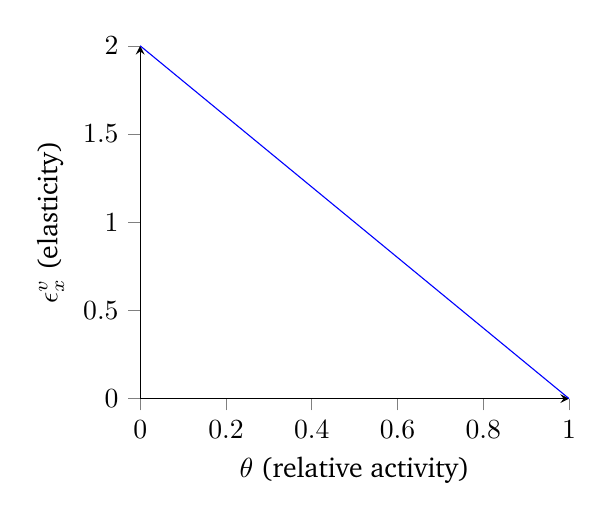
\begin{tikzpicture}
	\begin{axis}[width=200pt,axis x line=bottom, axis y line=left, tick align=outside, domain=0:1, xlabel=$\theta$ (relative activity), ylabel=$\epsilon_x^v$ (elasticity)]
		\addplot+[mark=none,smooth] (\x,{2 * (1 - \x)});
	\end{axis}
\end{tikzpicture}
\end{center}

Since $\theta$ represents the fraction of active enzyme, we see here that there is direct trade-off between the activity of the enzyme and the elasticity. It should be noted, that evolution can easily adjust $\theta$ for an individual enzyme by changing the $K_A$ or $K_I$ values, even without changing the concentration of the small-molecule effector (assuming it has other crucial functions in the cell). Therefore, evolution needs to weigh between how much of the enzyme is "wasted" by inhibition (or by inactivation), versus how much control it has on the flux. This can be viewed as a trade-off between the short-term goal of being able to adjust things quickly and the long-term goal of allocating resources efficiently in order to grow as fast as possible.

Another corollary of Equation \ref{eq:abs_elast} is that the control can be increased by changing the Hill coefficient ($h$). This could be a reason why mechanisms with very high cooperativity evolve for allosteric regulation \cite{Monod1965-dq}, as it increases elasticity without the added cost of losing enzyme activity.


\bibliographystyle{ieeetr}
\bibliography{control_theory}

\end{document}